\documentclass{auvsi_doc}
\setkeys{auvsi_doc.cls}{
	AUVSITitle={Design Summary},
%	AUVSIRevision=0.0,
%	AUVSIDescription={Created},
%	AUVSIAuthor={Kameron Eves},
%	AUVSIChecker={[Checker]},
	AUVSILogoPath={./figs/logo.pdf},
%	AUVSIDocID={AF-004}
}

% include extra packages, if needed
\usepackage{makecell}
\usepackage{multirow}
\usepackage{subcaption}

% Remove Heading Numbers
\setcounter{secnumdepth}{0}

\begin{document}
\begin{AUVSITitlePage}
\begin{artifacttable}
	\entry{TW-002, 0.1, 12-03-2018, Created, Kameron Eves, Andrew Torgesen}
	\entry{TW-002, 0.2, 12-10-2018, Added payload delivery sections, Andrew Torgesen, Kameron Eves}
	\entry{TW-002, 0.2, 12-10-2018, Reorganized after Dr. Jensen's Suggestions, Kameron Eves, Andrew Torgesen}
\end{artifacttable}
\end{AUVSITitlePage}


\section{ Introduction}

Each year, the Association for Unmanned Vehicle Systems International (AUVSI) hosts a Student Unmanned Aerial Systems (SUAS) competition. This year’s competition will be held June 12th to 15th, 2019 and BYU will be sending a team to compete.

The aircrafts entered into the competition are judged primarily on a demonstration of ability to autonomously complete a mission which includes the following tasks:

\begin{itemize}
	\item\textbf{Fly Waypoint Path} - Fly waypoints given to the the team just prior to the competition. In this process, and throughout the entire mission, the aircraft must avoid virtual obstacles and stay within boundaries (both horizontal and vertical).
	\item\textbf{Visual Target Classification} - Capture an image of several targets within a search area and report to the judges the shape, color, alpha-numeric character, alpha-numeric character color, and geolocation of each target.
	\item\textbf{Payload Delivery} - Drop on a specified location, an unmanned ground vehicle (UGV) that itself carries a small water bottle. Then, carrying its water bottle, the UGV must drive to a second specified location.
\end{itemize}

In order to accomplish these tasks, our team has decided upon the following objective statement:

\begin{quote}
Improve upon last year’s BYU AUVSI unmanned aerial system (UAS) by improving path planning, obstacle avoidance, visual object detection, and payload delivery by April 1, 2019 with a budget of \$3,500 and 2,500 man hours.
\end{quote}

We have stipulated several key success measures which are enumerated in Table~\ref{tab:key_measures}. Additional market requirements, performance measures, ideal values, and target values are included in RM-001.

\begin{table}[H]
	\centering
	\caption{Key success measures for the UAS}\label{tab:key_measures}
\begin{tabular}{|P{7.1cm}|>{\centering\arraybackslash}P{0.75cm}|>{\centering\arraybackslash}P{0.75cm}>{\centering\arraybackslash}P{0.75cm}>{\centering\arraybackslash}P{0.75cm}|>{\centering\arraybackslash}P{0.75cm}>{\centering\arraybackslash}P{0.75cm}>{\centering\arraybackslash}P{0.75cm}|}
	\multicolumn{8}{c}{\textbf{\underline{Key}}} \\
		\multicolumn{8}{l}{\textbf{Performance:} \textbf{SG} = Stretch Goal, \textbf{A} = Excellent,	\textbf{B} = Good,	\textbf{C} = Fair}  \\
		\multicolumn{8}{l}{\textbf{Acceptable:} \textbf{L} = Lower, \textbf{I} = Ideal,	\textbf{U} = Upper}\\
	\hline
	\rowcolor[HTML]{C0C0C0}
	 & \multicolumn{4}{c|}{\textbf{Performance}} &\multicolumn{3}{c|}{\textbf{Acceptable}}  \\\rowcolor[HTML]{C0C0C0}
	\multirow{-2}{*}{ \textbf{Measures (units)}} &{\textbf{SG}} & {\textbf{A}} & {\textbf{B}} & {\textbf{C}} & {\textbf{L}} & {\textbf{I}} & {\textbf{U}} \\

	\hline
	\textbf{Obstacles Hit (\#)} & 0 & 1 & 3 & 5 & 0 & 0 & 5 \\
	\hline
	\textbf{Average Waypoint Proximity (ft)} & 5 & 20 & 25 & 30 & 0 & 0 & 100 \\
	\hline
	\textbf{Characteristics Identified (\%)} & 80 & 40 & 30 & 20 & 20 & 100 & 100 \\
	\hline
	\textbf{Airdrop Accuracy (ft)} & 5 & 25 & 50 & 75 & 0 & 0 & 75 \\
	\hline
	\textbf{Number of Manual Takeovers (\#)} & 0 & 1 & 2 & 3 & 0 & 0 & 3 \\
	\hline
\end{tabular}
\end{table}


\section{Description of Design}
\subsection{Airframe}
The My Fly Dream Nimbus Pro airframe was selected as this year's airframe. With a wingspan of 1.95~m and fuselage capacity of 8,000~cc, it is significantly larger than last year's airframe. The new airframe boasts a design speed of 13~m/s, as modeled in XFLR5. This is a significant 35\% decrease from last year's plane. The new airframe also has a fuselage capacity of 8,000~cc: a 7\% increase over last year's plane. This is essential with the addition of a UGV as the required payload in this year's competition, especially since last year's plane didn't have room for even a water bottle inside the fuselage. As a final feature, the new airframe features easily removable wings and tail for easy and quick replacement in the case of a severe crash. This should help satisfy the fast and cheap assembly/rebuild prescribed on the Airframe Requirements Matrix (AF-001). See Fig. \ref{airframe} for a photo of the airframe, and Fig. \ref{components} for a photo of component placement within the airframe. See AF-002 for more detailed description of the airframe.

\begin{figure}[h!]
\centering
\begin{subfigure}[h]{.49\textwidth}
	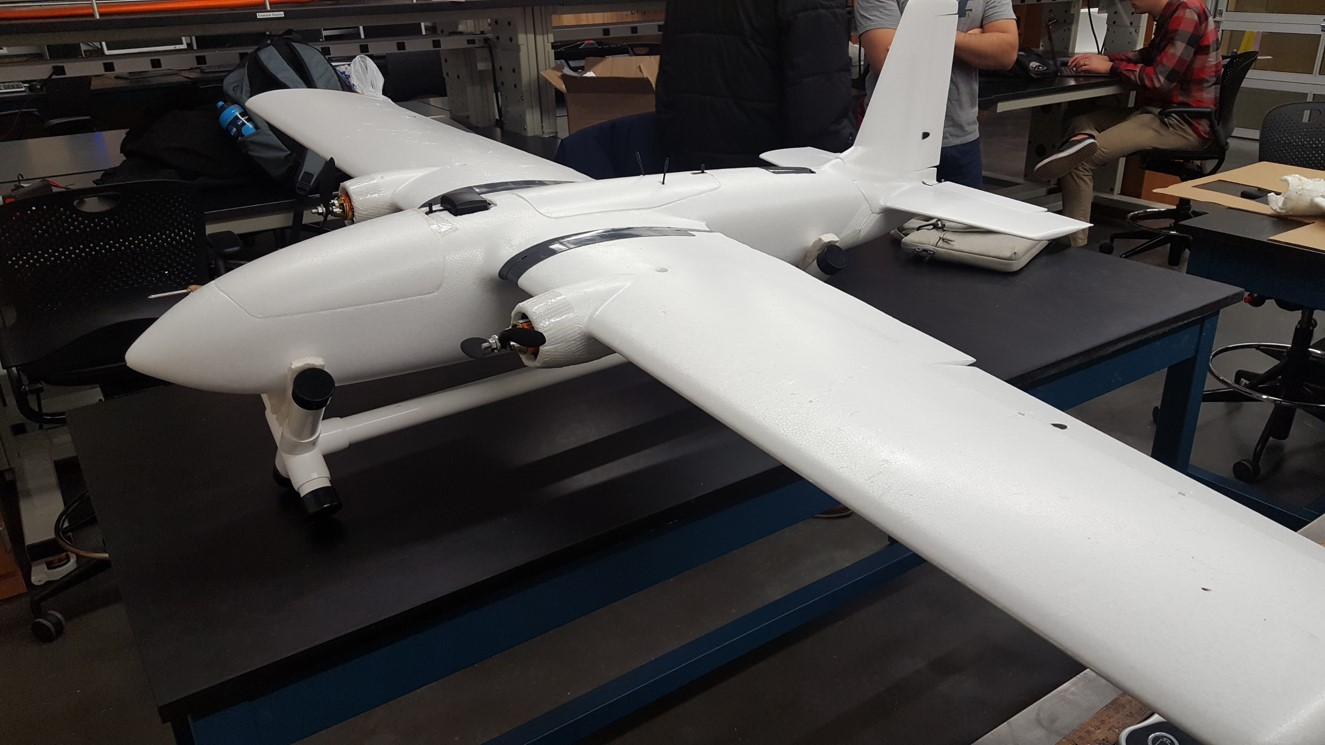
\includegraphics[width=1\linewidth]{figs/airframe.jpg}
	\centering
	\caption{The new airframe boasts a large wingspan, large fuselage, and easily removable wings and tail.}
	\label{airframe}
\end{subfigure}
\begin{subfigure}[h]{.49\textwidth}
	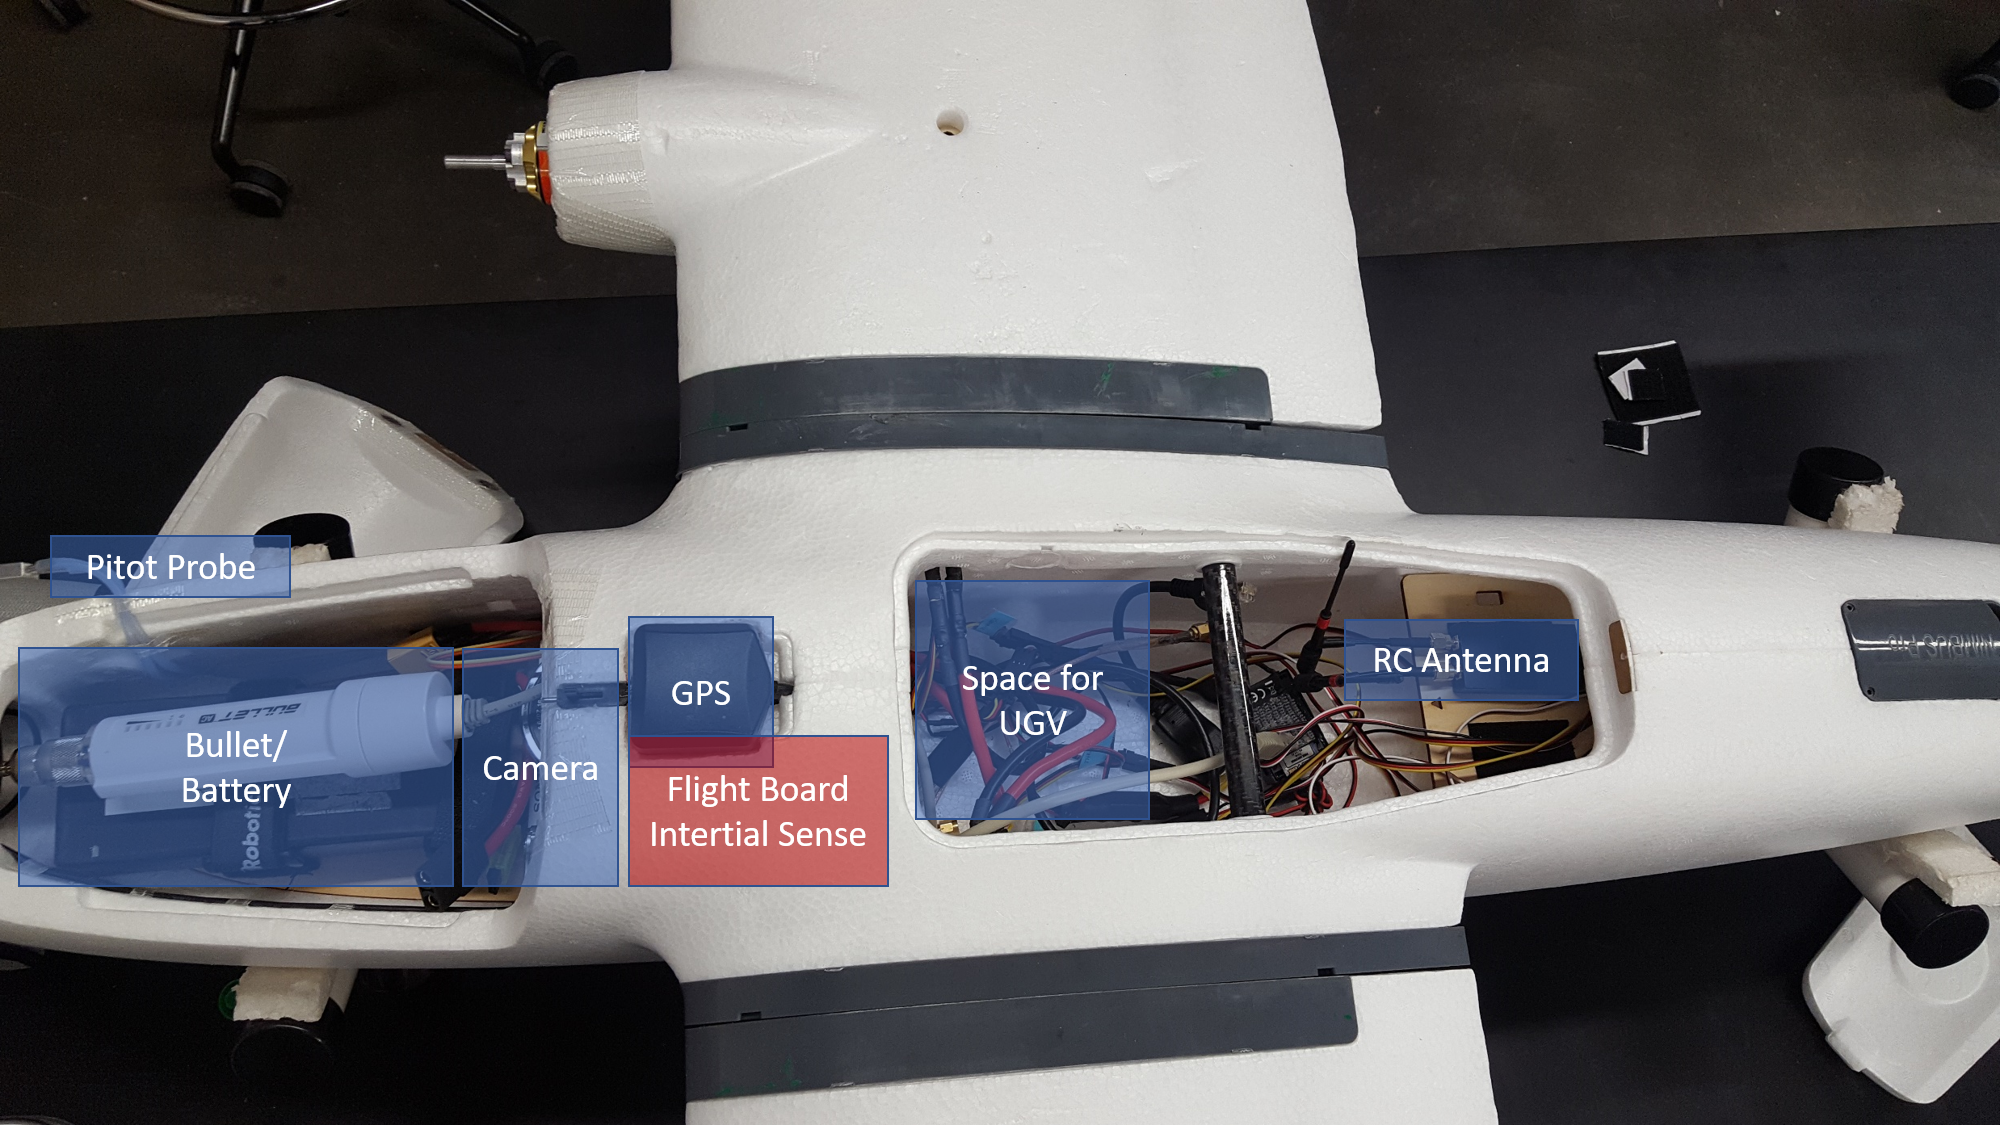
\includegraphics[width=1\linewidth]{figs/ComponentPlacement.png}
	\centering
	\caption{Component placement is relatively easy in the spacious fuselage. Components are labeled for clarity.}
	\label{components}
\end{subfigure}
\end{figure}

\subsection{Visual Target Classification}
This year's vision team is changing our system architecture for classifying targets which will allow for better communication and organization. Instead of downloading each image and image state onto someone's personal computer, the computer onboard the plane will send image and vehicle state data to a server on the ground. This server will have a compiled database of all images captured and will attach classification data onto each image as it is manually processed. Our autonomous detection script will also be querying the server image database and classifying
images. One team member will be monitoring the autonomous output ready to kill the
program if it is sending too many false positives (which cause the team to incur a
penalty). An autonomous classification system is being developed in parallel with manual system described above. This is a large task as each of the 6 characteristics we are required to identify could potentially be done using a different method of machine vision and/or machine learning. See CD-002 for a more detailed description of the visual target classification system design.
\subsection{Payload Delivery}
The UGV will be loaded within the aircraft. Given the desired drop location, the autopilot will determine the optimal direction and speed from which to drop the payload, using estimated airspeed conditions. A command from the autopilot will open a small hatch on the bottom of the plane and the UGV will fall out. Strings will attach the UGV to a lightweight fabric parachute with a hole in its center (for improved accuracy). The fabric parachute will be loaded onto the aircraft in a tube that will allow the UGV to pull it out of the aircraft as it falls. After exiting the aircraft, the parachute will be opened by drag. The drag caused by the fabric will slow down the system enough to allow the UGV to survive impact without damage.

\section{Summary of Expected Performance}

With the design discussed above we expect the following performance on our key success measures:

\begin{itemize}
	\item\textbf{Obstacles Hit} - The slower design speed of airframe will allow us to follow the path stipulated by our path planner more accurately and so avoid obstacles more effectively. This combined with a robust path planner design carried over from last year's design leads us to expect to achieve our stretch goal in this key success measures.
	\item\textbf{Average Waypoint Proximity} - Again, the slower design speed of airframe will allow us to follow the path stipulated by our path planner more accurately and so hit the waypoints more effectively this combined with a robust path planner design carried over from last year's design leads us to expect to achieve excellent performance in this key success measures.
	\item\textbf{Characteristics Identified} - The choose vision system architecture along with a new camera has significantly improve the effectiveness of our visual target classification. Improved camera resolution allows for more accurate manual characteristic identification, and the improved system flow reduces false positives. Thus far, we have developed a system capable of detecting targets with around 70\% accuracy. We have also modified a deep learning-based character recognition system to detect synthetic letters with over 90\% accuracy. Thus we expect to achieve excellent performance in this key success measures.
	\item\textbf{Airdrop Accuracy} - As part of the design process, we have considered multiple points of failure and used those points to inform our design. This, along with the testing documented in GV-003 and GV-004, give us confidence that we can achieve an airdrop accuracy within 25 feet from the target drop location. This falls within the range of excellent performance for this key success measure.
	\item\textbf{Number of Manual Takeovers} - The airframe, including it's slower design speed and high quality craftsmanship, will improve our aircrafts ability to stay within boundaries and avoid rule violations this will minimize rule violations. From the testing of our airframe detailed in AF-004 we feel confidant that we will be able to achieve our stretch goal in this key success measure.
\end{itemize}

\section{Status and Future Plans}
The entire system is very close to being ready for a mock competition which we will perform first thing next semester.The airframe is currently ready for RC flight testing. Essential components for RC flight have been installed and balanced for the optimal CG placement (as determined using the XFLR5 model), and we have tentative plans for installing the remaining components. The system for manual target recognition is mostly complete and almost ready for inflight testing. The new camera's interface with the system has yet to be built, however there is a strong framework in place for saving and accessing pictures from the server. We have also constructed a draft of the user interface that contacts the server and requests images and sends back cropped and classified images back to the server. As of right now, we have converged on a method, built a prototype, and tested the software and hardware from last year's system on the ground, but not in the air. The new mechanism for releasing the UGV has not yet been constructed and is the next big step our team must take. In the mock competition we will test last years system to ensure we understand the complexities of the problem.

Much of the requisite work work on the airframe and manual target classification system is complete. Further testing remains to be done to determine if wing extensions will be necessary. This will probably consist mostly of imaging tests. If image quality is unsatisfactory, then efforts to reduce the design speed by extending the wings will be worthwhile. Otherwise, our time may be better used elsewhere. In the future, we will also be working on testing the character recognizer on real images of targets and be developing the automated shape classifier and color recognition systems. The biggest task remaining for our team is building the new payload delivery system. Now that the airframe specifications are known, including a dedicated space in the fuselage for the UGV, we can begin construction and testing next semester. This will include iterating the combined payload delivery system (drop calculation algorithm, parachute, and UGV) with repeated simulation and hardware testing to ensure repeatability of expected performance in the face of differing environmental conditions, such as wind speed and direction.

\section{Conclusion}
From our design work outlined above and expounded upon in the artifacts below, we are confident that we will be able to construct and refine a product capable of meeting all of our key success measures and performing well in the AUVSI competition.
% document contents
\end{document}
